%%% -*- TeX-engine: xetex -*-
\documentclass{beamer}

% for themes, etc.
\usepackage{times}  % fonts are up to you
\usepackage{graphicx}
\usepackage{color}
\mode<presentation>
{
 \usetheme{Copenhagen}
 \usecolortheme{seahorse}
}
\usepackage{xeCJK}
\setCJKmainfont{WenQuanYi Micro Hei}

\title{基于翻译技术的流量调度}
\author{王文鑫}
\date{2016年1月15日}
\AtBeginSection[]
{
  \begin{frame}<beamer> 
    \tableofcontents[currentsection]
  \end{frame}
}

\begin{document}

\begin{frame}
  \titlepage
\end{frame}

\section{背景介绍}
\subsection{MAP-T}

\begin{frame}
  \frametitle{MAP-T}

  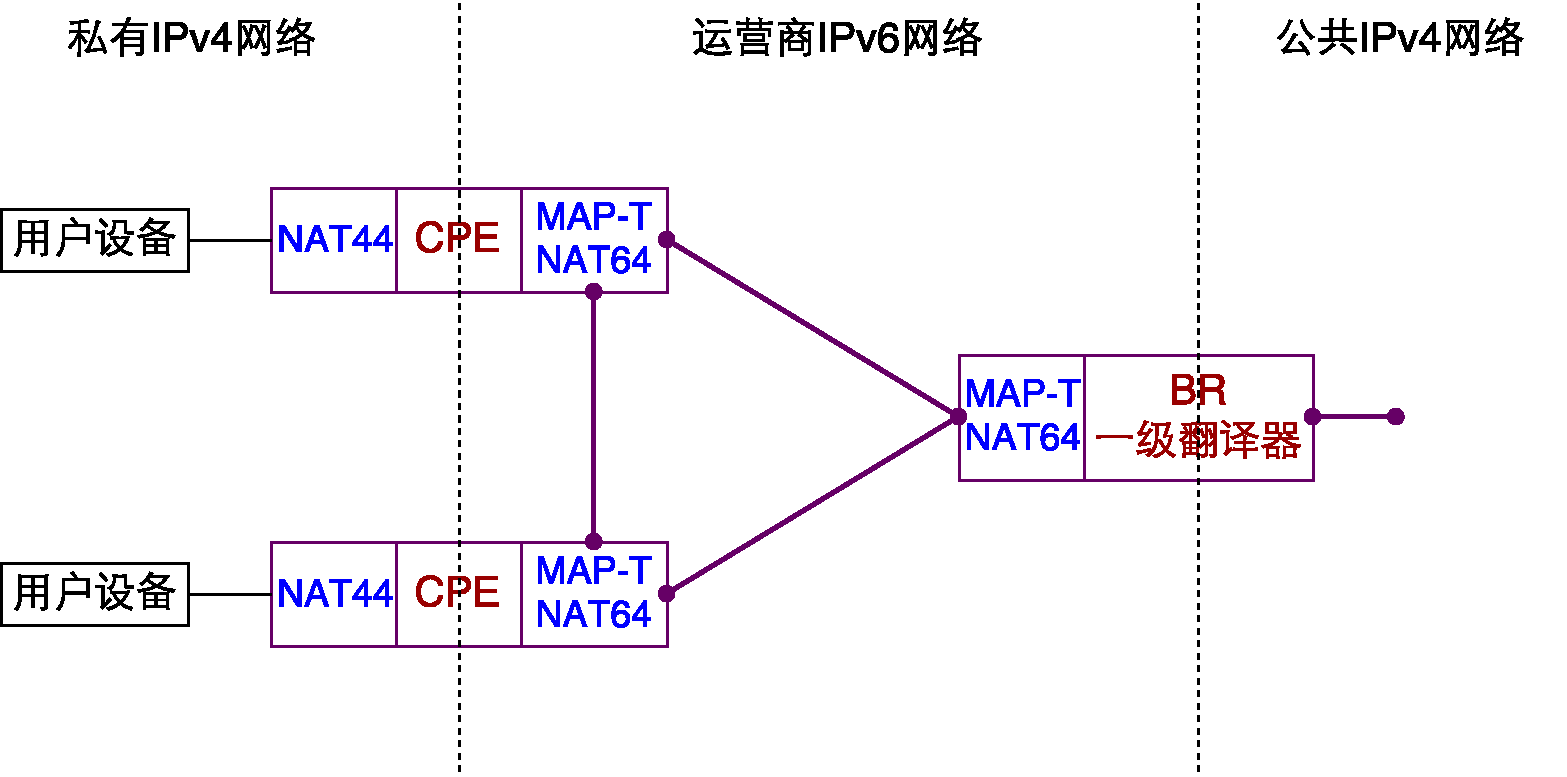
\includegraphics[width=\textwidth]{figs/MAP-T.pdf}  
  \vspace{1.5em}
  使用IPv6网络,将内部IPv4网络与公共IPv4网络相连
\end{frame}

\begin{frame}
  \frametitle{Mapping of Address and Port Using Translation}

  \begin{block}{做法}
    \begin{itemize}
    \item 在IPv6网络上传输IPv4数据包
    \item 使用固定的端口划分和分配共享全局地址
    \item 每个CPE获取一段全局地址的端口,进行私有IPv4地址到全局IPv4地址的端口映射
    \item 使用一个特定的IPv6前缀翻译进出口的数据包,通过路由引向BR
    \end{itemize}
  \end{block}

  \begin{block}{优点}
    \begin{itemize}
    \item 实现对全局地址的共享
    \item 私有到全局地址的映射状态分布在各个CPE上
    \item 一级翻译器(BR)无需维护每个连接的映射状态
    \end{itemize}
  \end{block}

\end{frame}

\begin{frame}
  \frametitle{Mapping of Address and Port Using Translation}

  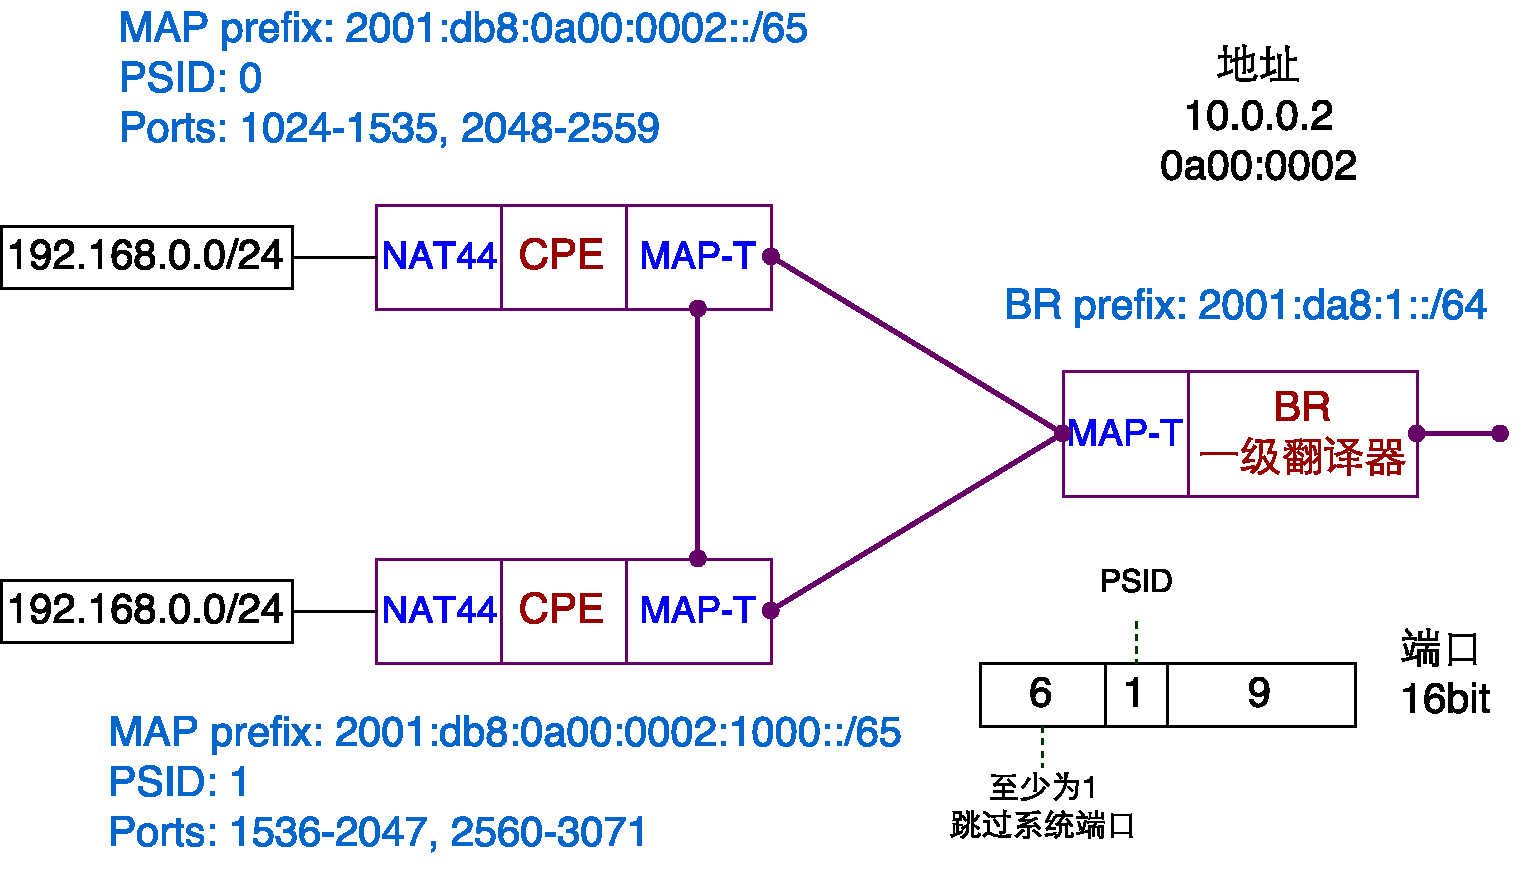
\includegraphics[width=\textwidth]{figs/MAP-T-details.pdf}  
\end{frame}

\subsection{高复用比带来的问题}

\begin{frame}
  \frametitle{高复用比带来的问题}

  \begin{itemize}
  \item 每个CPE可以用来进行映射的端口数有限
  \item 一旦这些端口耗尽,就无法为新连接提供映射
  \end{itemize}
\end{frame}

\begin{frame}
  \frametitle{解决方法}
  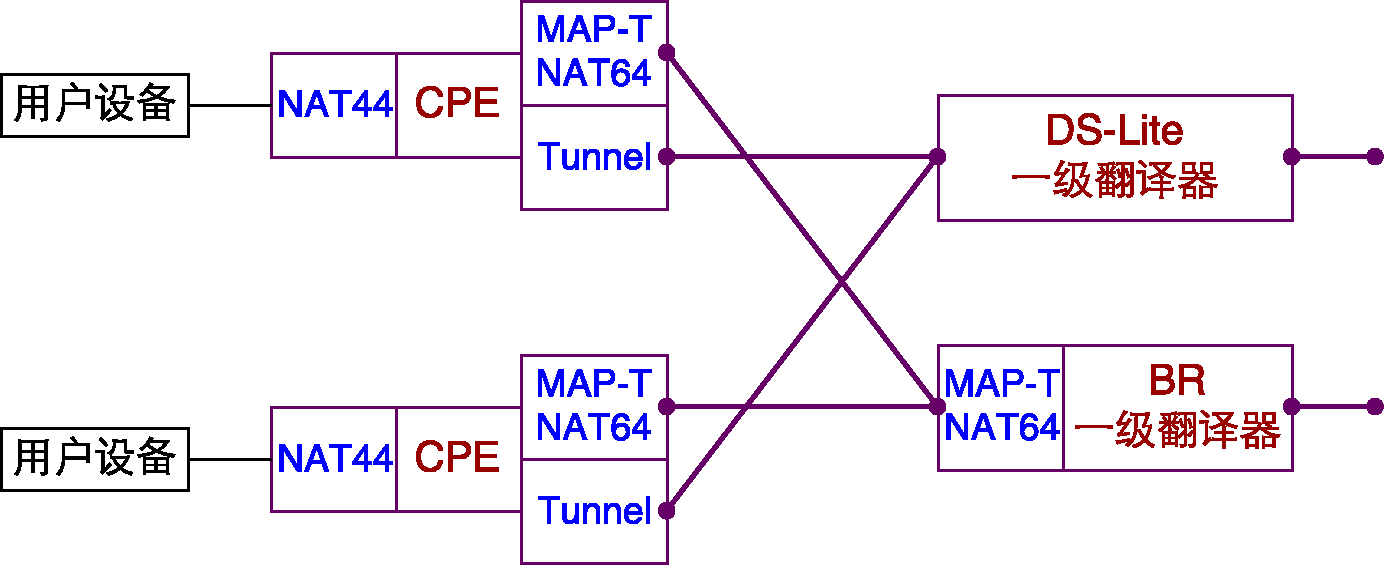
\includegraphics[width=\textwidth]{figs/MAP-T-DS-Lite.pdf}  

  转而使用粒度更细、复用比更高的翻译/封装机制,如DS-Lite
\end{frame}

\section{研究目标}
\subsection{研究目标}
\begin{frame}
  \frametitle{研究目标}

  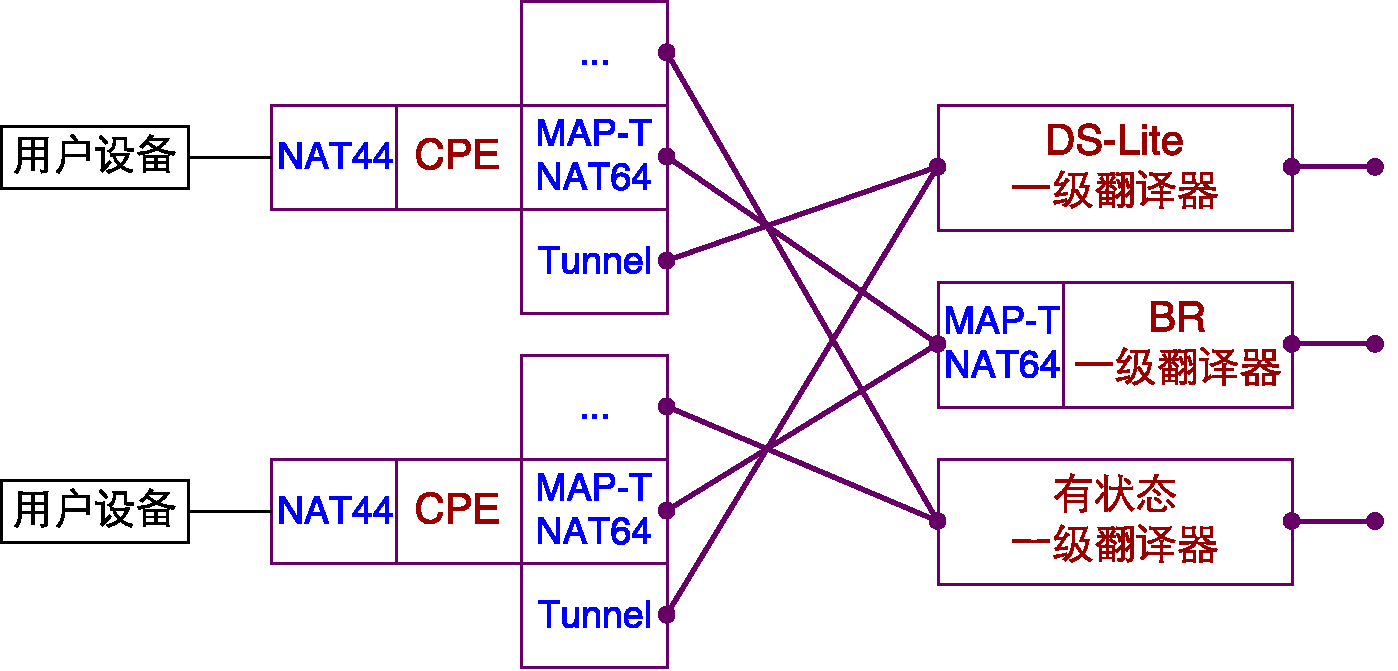
\includegraphics[width=\textwidth]{figs/MAP-T-Multiple-DS-Lite.pdf}  
  \vspace{1.5em}
  引入多个有状态的一级翻译机,在这些翻译机间调度超出复用比额度的流量
\end{frame}

\begin{frame}
  \frametitle{目的}
  \begin{itemize}
  \item 负载均衡
  \item 容错
  \item 特定路由策略
    \begin{itemize}
    \item 根据目的地,选择在某个运营商出口的翻译机
    \item 为某些网络应用单独分配翻译机
    \end{itemize}
  \item 调度算法也许可以用于多个MAP-T一级翻译机的场景
  \end{itemize}
\end{frame}

\section{研究路线}
\subsection{工作划分}

\begin{frame}
  \frametitle{工作划分}
  \begin{block}{算法}
    \begin{itemize}
    \item 选择算法:决定某个数据包使用的翻译器
      \begin{itemize}
      \item 在CPE上完成
      \end{itemize}
    \item 分配算法:决定某个CPE可以使用的翻译器集合
    \end{itemize}
  \end{block}
\end{frame}

\subsection{选择算法}

\begin{frame}
  \frametitle{选择算法:决定某个数据包使用的翻译器}
  \begin{columns}
    \column{0.5\textwidth}
    \begin{block}{类比4层负载均衡器}
      \begin{itemize}
      \item 轮询
      \item 最小连接数
      \item 加权
        \begin{itemize}
        \item 轮询
        \item 最小连接数
        \end{itemize}
      \item 地址哈希
        \begin{itemize}
        \item 需要处理地址非均匀分布的情况
        \end{itemize}
      \end{itemize}
    \end{block}
    \column{0.5\textwidth}
    \begin{figure}[ht]
    \begin{center}
      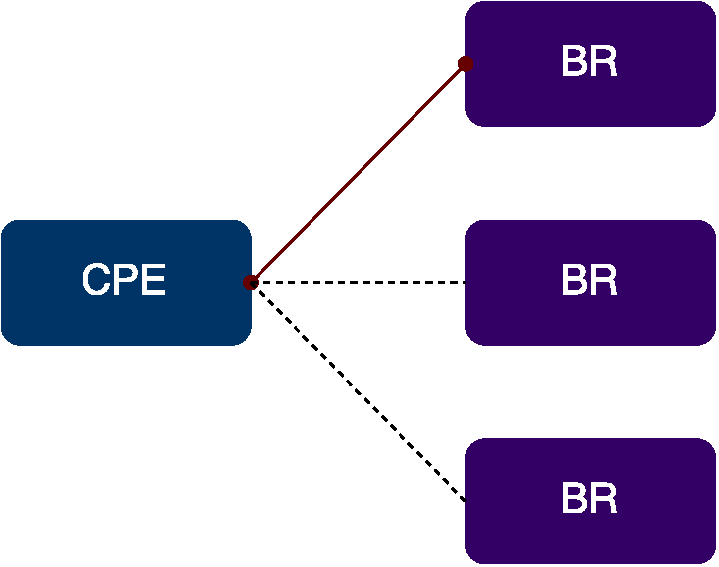
\includegraphics[width=15em]{figs/BR-selection.pdf}  
    \end{center}
    \end{figure}
  \end{columns}
\end{frame}

\begin{frame}
  \frametitle{选择算法}
  \begin{columns}
    \column{0.5\textwidth}
    \begin{block}{特定的路由策略}
      \begin{itemize}
      \item 将有特定目的的一级翻译器分成不同的策略组
        \begin{itemize}
        \item 电信组、优库组……默认组
        \end{itemize}
      \item 每个流匹配到一个策略组内
      \item 若组内有多个翻译器,则继续负载均衡
      \end{itemize}
    \end{block}
    \column{0.5\textwidth}
    \begin{figure}[ht]
      \begin{center}
        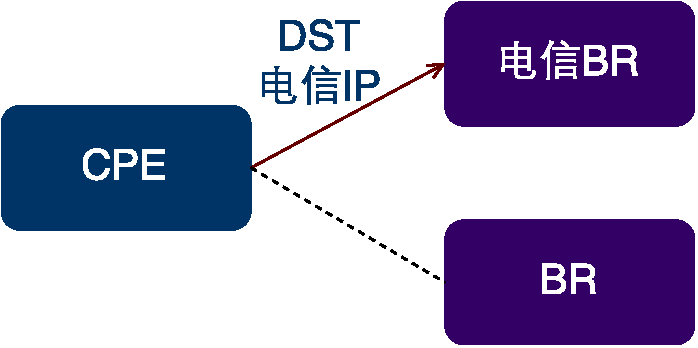
\includegraphics[width=15em]{figs/BR-selection-policy.pdf}  
      \end{center}
    \end{figure}
  \end{columns}
\end{frame}

\begin{frame}
  \frametitle{选择算法}
  \begin{block}{难点}
    \begin{itemize}
    \item 有效性
    \item 与分配算法的配合度
    \item 对于有连接的传输协议(TCP),保证某个流的所有包通过相同的翻译器
    \end{itemize}
  \end{block}
\end{frame}

\subsection{分配算法}

\begin{frame}
  \frametitle{分配算法:CPE共享所有翻译器}
  \begin{columns}
    \column{0.5\textwidth}
    \begin{itemize}
    \item 依赖CPE的选择算法进行负载均衡
    \item 无法根据一级翻译器的状态进行调整
    \item 性能并不一定差,可以作为参考算法
    \end{itemize}
    \column{0.5\textwidth}
    \begin{figure}[ht]
      \begin{center}
        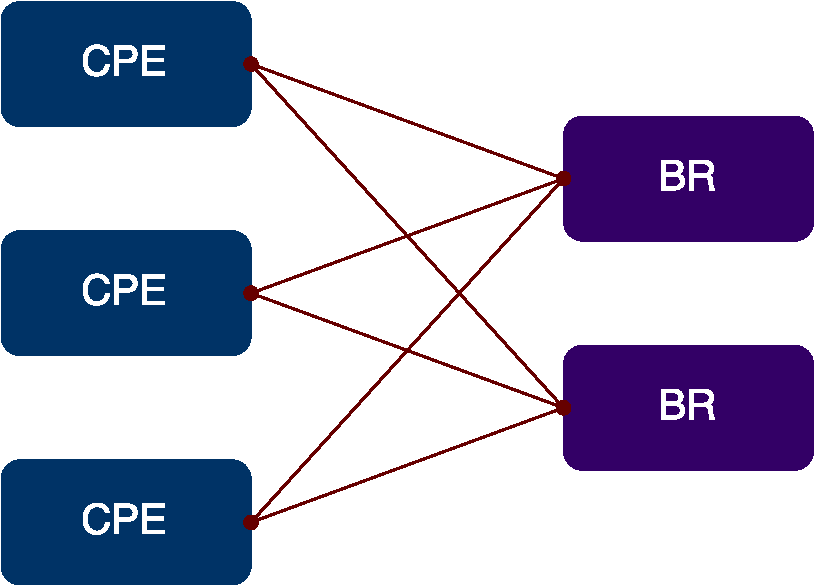
\includegraphics[width=15em]{figs/BR-delegation-shared.pdf}  
      \end{center}
    \end{figure}
  \end{columns}
\end{frame}

\begin{frame}
  \frametitle{分配算法:在CPE间静态分配翻译器}
  \begin{columns}
    \column{0.5\textwidth}
    \begin{itemize}
    \item 在配置CPE时指定可以使用的翻译器
    \item 无法使用其它CPE得到的翻译器
      \begin{itemize}
      \item 即便它们是空闲的
      \item 即便本CPE分配到的翻译器出错
      \end{itemize}
    \end{itemize}
    \column{0.5\textwidth}
    \begin{figure}[ht]
      \begin{center}
        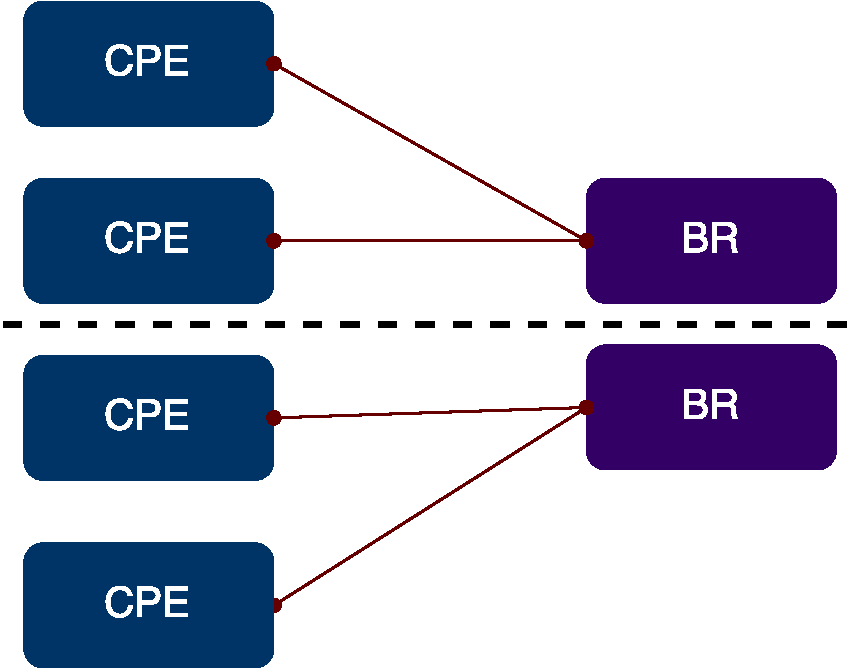
\includegraphics[width=15em]{figs/BR-delegation-static.pdf}  
      \end{center}
    \end{figure}
  \end{columns}
\end{frame}

\begin{frame}
  \frametitle{分配算法:在CPE间动态分配翻译器}
  \begin{columns}
    \column{0.5\textwidth}
  \begin{block}{引入中心控制器}
    \begin{itemize}
    \item 获取各个一级翻译器的状态
    \begin{itemize}
    \item e.g. SNMP
    \end{itemize}
    \item 为各个CPE分配翻译器
    \begin{itemize}
    \item e.g. DHCP信令
    \end{itemize}
    \item 当翻译器的负载/状态发生变化时,重新分配
    \end{itemize}
  \end{block}
    \column{0.5\textwidth}
    \begin{figure}[ht]
      \begin{center}
        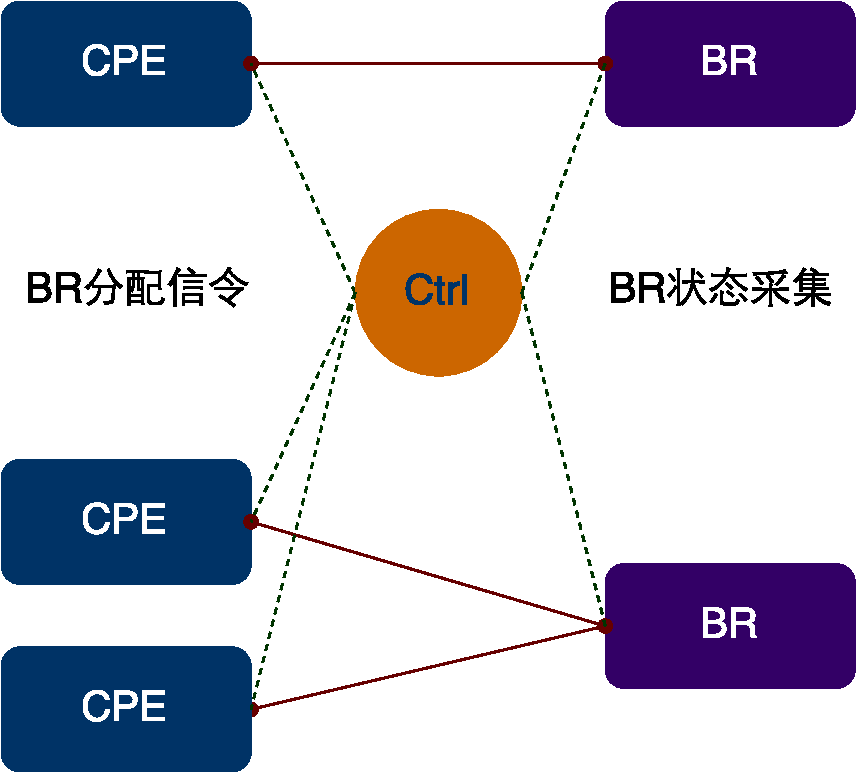
\includegraphics[width=15em]{figs/BR-delegation-centralized.pdf}  
      \end{center}
    \end{figure}
  \end{columns}
\end{frame}

\begin{frame}
  \frametitle{分配算法:在CPE间动态分配翻译器}
  \begin{block}{中心控制器的好处}
    \begin{itemize}
    \item 类似于SDN中,控制器掌握所有路由器的状态,统一控制路由走向
    \item 控制器掌握所有翻译器的状态,对出口流量进行统一调度
    \item 否则,由各个CPE单独获取翻译器状态,并协调分配
      \begin{itemize}
      \item 效率低,收敛慢
      \end{itemize}
    \end{itemize}
  \end{block}
\end{frame}

\begin{frame}
  \frametitle{分配算法:难点}
  \begin{itemize}
  \item 结合选择算法,使得无论整体负载稳定与否,各翻译器间的负载尽量达到均衡
  \item 在平稳状态下,各翻译器的负载应当较为稳定,不应抖动
  \item 对于有连接的传输协议(TCP),即便某个CPE分配到的翻译器集合发生变化,当前未结束的流的路由应该保持不变
  \end{itemize}
\end{frame}

\section{进度安排}

\begin{frame}
  \frametitle{进度安排}
  \begin{itemize}
  \item 1月16日-2月29日:项目代码阅读和整理,对当前流量特性进行测量和分析
  \item 3月1日-中期审查:翻译器选择算法设计和实现
  \item 中期审查-5月20日:翻译器分配算法设计和实现
  \item 5月20日-6月5日:整体算法的性能测量
  \item 6月5日-答辩:论文完善及答辩准备
  \end{itemize}
\end{frame}

\section{参考文献}
\begin{frame}
  \frametitle{参考文献}
  \begin{itemize}
  \item \href{https://tools.ietf.org/html/rfc7599}{RFC7599}
  \item \href{https://tools.ietf.org/html/rfc7597}{RFC7597}
  \item \href{https://tools.ietf.org/html/rfc7598}{RFC7598}
  \item \href{https://tools.ietf.org/html/rfc6052}{RFC6052}
  \item
    \href{https://wiki.opendaylight.org/images/4/42/OpenDaylight-lb-prj-prop-v3.pdf}{OpenDaylight Project Proposal “Dynamic Flow Management”}
  \item
    \href{http://www.cisco.com/c/en/us/support/docs/interfaces-modules/content-switching-module/28580-lb-algorithms.html}{Understanding CSM Load Balancing Algorithms}
  \end{itemize}
\end{frame}
\end{document}
